% !TEX root = relatorio.tex
%
% Capítulo 5 — Testes e Validação
%
\chapter{Testes e Validação} \label{cap:testes}

A validação do Play4Change assenta em quatro camadas complementares: testes unitários que verificam o comportamento isolado do domínio e dos serviços de aplicação, testes de integração que exercitam a camada HTTP em contexto Spring parcial, testes de segurança que confrontam as defesas com os vectores de ataque identificados na análise de risco (§\ref{sec:riscos}), e um questionário de usabilidade aplicado a doze utilizadores reais. Juntas, estas camadas cobrem 49 ficheiros de teste distribuídos pelos módulos \textit{server} e \textit{play4change-web}.

% ─────────────────────────────────────────────────────────────────────────────
\section{Estratégia de Testes} \label{sec:estrategia-testes}

A estratégia decorre diretamente das decisões de arquitetura do sistema e assenta em três princípios: (1)~\textbf{isolamento total pelo padrão hexagonal} --- todas as dependências externas (repositórios, portas de e-mail, publicadores de eventos, geradores de IA) são interfaces, substituídas em cada teste unitário por duplicados \textit{Mockk}, pelo que os testes de domínio executam em memória pura, na ordem dos microssegundos; (2)~\textbf{\texttt{Either<Error, T>} como contrato de resultado} --- a biblioteca Arrow impõe que cada caso de uso devolva \texttt{Either<DomainError,~T>} em vez de lançar exceções, e os testes inspeccionam o tipo concreto do erro, tornando os casos de insucesso tão verificáveis como os de sucesso; e (3)~\textbf{separação clara dos três níveis}, conforme a Tabela~\ref{tab:suite-nivel}.

\begin{table}[htb]
\centering
\caption{Níveis da suite de testes automatizados.}
\label{tab:suite-nivel}
\begin{tabular}{@{}llll@{}}
\toprule
\textbf{Nível} & \textbf{Ferramenta principal} & \textbf{Contexto Spring} & \textbf{Dependências externas} \\
\midrule
Unitário   & JUnit~5 + Mockk         & Nenhum               & Todas em mock \\
Integração & @WebMvcTest + MockMvc   & Parcial (camada web) & Serviços em mock \\
Segurança  & JUnit~5 + @WebMvcTest   & Parcial ou nenhum    & Todas em mock \\
\bottomrule
\end{tabular}
\end{table}

No frontend (React/Vite), os testes de componente e de utilitários utilizam \textit{Vitest} com \textit{React Testing Library}. A Tabela~\ref{tab:suite-dimensao} resume a dimensão total da suite.

\begin{table}[htb]
\centering
\caption{Dimensão da suite de testes por módulo.}
\label{tab:suite-dimensao}
\begin{tabular}{@{}llll@{}}
\toprule
\textbf{Módulo} & \textbf{Ficheiros de teste} & \textbf{Linguagem} & \textbf{Ferramenta} \\
\midrule
Servidor — aplicação, domínio e infra & 25 & Kotlin     & JUnit~5 + Mockk \\
Servidor — camada web / integração    & 11 & Kotlin     & @WebMvcTest + MockMvc \\
Frontend — componentes e utilitários  & 13 & TypeScript & Vitest + RTL \\
\midrule
\textbf{Total} & \textbf{49} & & \\
\bottomrule
\end{tabular}
\end{table}

% ─────────────────────────────────────────────────────────────────────────────
\section{Testes Unitários} \label{sec:testes-unitarios}

\subsection{Objetos de Valor — \texttt{Name}} \label{sec:testes-vos}

O \texttt{Name} é o objeto de valor que representa o nome de perfil de um utilizador, construído pelo método de fábrica \texttt{Name.create(raw:~String?)}. O \texttt{NameValidationTest.kt} (8 testes) cobre nulos, entradas só de espaços, comprimentos fora do intervalo 2--100 e caracteres de controlo, conforme a Tabela~\ref{tab:name-testes}.

\begin{table}[htb]
\centering
\caption{Casos de teste do objeto de valor \texttt{Name}.}
\label{tab:name-testes}
\begin{tabular}{@{}lll@{}}
\toprule
\textbf{Caso} & \textbf{Entrada} & \textbf{Resultado esperado} \\
\midrule
Null               & \texttt{null}            & \texttt{Result.Failure} \\
Só espaços         & \texttt{"\ \ \ "}         & \texttt{Result.Failure} \\
Comprimento 1      & \texttt{"A"}             & \texttt{Result.Failure} \\
Comprimento 101    & \texttt{"A"~$\times$~101} & \texttt{Result.Failure} \\
Caracter de controlo & \texttt{"Alice\textbackslash u0000Bob"} & \texttt{Result.Failure} \\
Comprimento 2 (limite inf.) & \texttt{"Al"}   & \texttt{Result.Success} \\
Comprimento 100 (limite sup.) & \texttt{"A"~$\times$~100} & \texttt{Result.Success} \\
Válido             & \texttt{"Alice"}         & \texttt{Result.Success("Alice")} \\
\bottomrule
\end{tabular}
\end{table}

\subsection{Autenticação — \texttt{TokenService} e \texttt{MagicLinkService}} \label{sec:testes-auth}

O \texttt{TokenServiceTest.kt} (2 testes) valida a revogação de família de tokens JWT: quando um token de actualização é revogado, toda a família (\texttt{familyId}) é invalidada, protegendo contra reutilização em caso de roubo (ameaça R04, §\ref{sec:riscos}); a revogação de um token inexistente é silenciosa, sem chamadas indevidas.
O \texttt{MagicLinkServiceTest.kt} (7 testes) cobre o ciclo completo do fluxo \textit{magic link}: o token em claro nunca é guardado na base de dados (apenas o SHA-256); \texttt{claimToken} é um \texttt{UPDATE~\ldots~WHERE~used=false} atómico, pelo que um segundo consumo concorrente falha; e a conta é criada automaticamente na primeira verificação bem-sucedida.

\subsection{Baralhagem Anti-fraude e Cadência de Entrega} \label{sec:testes-tasks}

O \texttt{AntiCheatShuffleTest.kt} (5 testes) valida a baralhagem determinística de opções (§\ref{sec:atribuicao}), usando \texttt{(userId, taskId, enrollmentId)} como semente: o mesmo utilizador vê sempre a mesma ordem, utilizadores distintos recebem ordens distintas, o índice da resposta correta é sempre mapeado correctamente, e a permutação é uma bijecção.

O \texttt{TaskDeliveryRateTest.kt} (6 testes) valida os dois modos de operação e o guarda de arranque, que lança \texttt{IllegalStateException} se detetar \texttt{devMode=true} com perfil \texttt{prod} ativo. O \texttt{EnrollmentPrerequisiteGateTest.kt} (6 testes) confirma que o \texttt{EnrollmentService} recusa inscrições com pré-requisitos incompletos.

\subsection{Gestão de Tópicos e Detecção de Ciclos no DAG} \label{sec:testes-topicos}

O \texttt{TopicPrerequisiteServiceTest.kt} (12 testes) valida a detecção de ciclos no grafo de pré-requisitos por pesquisa em profundidade (DFS) --- ciclo direto, ciclo transitivo e grafo válido --- bem como a rejeição de auto-ciclos e referências a tópicos inexistentes.

O \texttt{GenerationPhaseTransitionTest.kt} (9 testes) valida cada transição da máquina de estados \texttt{GenerationPhase} (\texttt{INGESTION~$\to$~ANALYSIS~$\to$~GENERATION~$\to$~INDEXING~$\to$~ACTIVE}), incluindo a recuperação após falha (\texttt{GENERATION~$\to$~FAILED~$\to$~INGESTION}).

\subsection{Deteção e Escalamento de Dificuldades} \label{sec:testes-struggle-unit}

O \texttt{StruggleDetectionTest.kt} (3 testes) verifica que qualquer resposta errada despoleta imediatamente a criação assíncrona de uma sessão de dificuldade. O \texttt{StruggleResolutionTest.kt} (4 testes) valida o ciclo de vida da \texttt{StruggleSession}: submissão parcial (\texttt{OPEN}), aprovação total (\texttt{RESOLVED}) e falha total com \texttt{depth}~$\geq$~\texttt{MAX\_STRUGGLE\_DEPTH} (escalamento para explicação). O \texttt{ErrorPatternClassifierTest.kt} (8 testes) valida a classificação por prioridade estrita --- \texttt{TIME\_PRESSURE} $>$ \texttt{READING\_ERROR} $>$ \texttt{WRONG\_CONCEPT}.

% ─────────────────────────────────────────────────────────────────────────────
\section{Testes de Integração} \label{sec:testes-integracao}

Os testes de integração arrancam um contexto Spring parcial (\texttt{@WebMvcTest}) e exercitam a camada HTTP completa --- serialização JSON, filtros de segurança, validação de \textit{beans} e tratamento de erros --- com os serviços de aplicação em mock.

\subsection{Limitação de Taxa — \texttt{RateLimitTest}} \label{sec:testes-rate-int}

O teste de integração mais sofisticado da suite: o contexto inclui o \texttt{SecurityConfig} e o \texttt{RateLimitService} reais (Bucket4j), mas substitui o \texttt{TimeMeter} por um \texttt{ManualTimeMeter} que avança o relógio programaticamente. Quatro casos são cobertos: limite estrito (5 pedidos $\to$ 202; 6.º $\to$ 429); reset de janela temporal ao avançar 11 minutos; isolamento por IP; e presença do cabeçalho \texttt{Retry-After} na resposta 429.

\subsection{Controlo de Acesso ao Swagger} \label{sec:testes-swagger}

O \texttt{SwaggerAccessControlTest.kt}, activado em dois perfis Spring distintos, valida a política de acesso à documentação da API (Tabela~\ref{tab:swagger-acesso}).

\begin{table}[htb]
\centering
\caption{Matriz de acesso ao Swagger UI testada por \texttt{SwaggerAccessControlTest}.}
\label{tab:swagger-acesso}
\begin{tabular}{@{}llll@{}}
\toprule
\textbf{Perfil} & \textbf{Papel} & \textbf{HTTP esperado} & \textbf{Verificação} \\
\midrule
default (dev) & nenhum & não é 401 nem 403 & \texttt{status != 401 \&\& status != 403} \\
prod          & nenhum & 401                & \texttt{status().isUnauthorized()} \\
prod          & USER   & 403                & \texttt{status().isForbidden()} \\
prod          & ADMIN  & não é 401 nem 403  & \texttt{status != 401 \&\& status != 403} \\
\bottomrule
\end{tabular}
\end{table}

\subsection{Controladores REST} \label{sec:testes-controllers}

Nove ficheiros \texttt{@WebMvcTest} (mais o \texttt{RateLimitTest.kt}, §\ref{sec:testes-rate-int}) cobrem os endpoints principais, sumariados na Tabela~\ref{tab:controllers-testes}.

\begin{table}[htb]
\centering
\caption{Cobertura dos testes de integração por controlador REST.}
\label{tab:controllers-testes}
\resizebox{\textwidth}{!}{%
\begin{tabular}{@{}ll@{}}
\toprule
\textbf{Controlador} & \textbf{Casos testados} \\
\midrule
\texttt{AdminTopicPrerequisiteController} & GET pré-requisitos, POST com ciclo, POST sem ciclo, grafo de aprendizagem, 404 \\
\texttt{StruggleController}               & GET sessão ativa, submissão de tarefa adaptativa, autenticação obrigatória \\
\texttt{TaskReportController}             & Criar relatório, correcção pelo admin, dismissal, listagem por tópico \\
\texttt{UserPreferencesController}        & Língua (BCP~47) e fuso horário (ZoneId) — válidos e inválidos \\
\texttt{UserProfileController}            & GET perfil, PATCH com nome válido e inválido \\
\texttt{BadgeController}                  & Crachás do utilizador, estatísticas de admin \\
\texttt{AdminTaskController}              & Estatísticas de tarefa, tarefas com dificuldade, actualização em lote \\
\texttt{TopicController}                  & Campo \texttt{currentPhase} no GET de admin, conteúdo do \texttt{generationLog} \\
\texttt{SwaggerAccessControlTest}         & Acesso sem autenticação em perfil padrão; 401/403/200 em perfil \texttt{prod} por papel \\
\texttt{AuthControllerValidationTest}     & Formato de e-mail, token de verificação inválido \\
\bottomrule
\end{tabular}%
}
\end{table}

\subsection{Frontend — Vitest + React Testing Library} \label{sec:testes-frontend}

Treze ficheiros de teste cobrem componentes, \textit{hooks}, adaptadores de dados e utilitários de validação (Tabela~\ref{tab:frontend-testes}).

\begin{table}[htb]
\centering
\caption{Ficheiros de teste do frontend (Vitest + RTL).}
\label{tab:frontend-testes}
\resizebox{\textwidth}{!}{%
\begin{tabular}{@{}ll@{}}
\toprule
\textbf{Ficheiro} & \textbf{O que valida} \\
\midrule
\texttt{ProtectedRoute.test.tsx}  & Redirecionamento de utilizadores não autenticados para \texttt{/login} \\
\texttt{validators.test.ts}       & Formato de e-mail, URL, lista de URLs (1–5), ficheiro PDF (tipo + tamanho $\leq$ 100~MB) \\
\texttt{useTopics.test.ts}        & Estado de carregamento, erro e dados do hook \texttt{useTopics} \\
\texttt{mockTopicAdapter.test.ts} & Fidelidade dos adaptadores de dados em mock \\
\texttt{LoginPage.test.tsx}       & Submissão de formulário, mensagens de erro \\
\texttt{AuthVerifyPage.test.tsx}  & Verificação de token da URL, estados de carregamento \\
\texttt{CreateTopicPage.test.tsx} & Validação de formulário, submissão com sucesso \\
\texttt{UserList.test.tsx}        & Renderização de lista, filtros \\
\texttt{PromoteUser.test.tsx}     & Confirmação de promoção, feedback visual \\
\texttt{BadgeOverview.test.tsx}   & Renderização de crachás e contagens \\
\texttt{ReportList.test.tsx}      & Listagem, filtro por estado \\
\texttt{ReportDetail.test.tsx}    & Detalhe de relatório, ações de admin \\
\texttt{formatters.test.ts}       & Formatação de datas, pontos e níveis de audiência \\
\bottomrule
\end{tabular}%
}
\end{table}

% ─────────────────────────────────────────────────────────────────────────────
\section{Testes de Segurança} \label{sec:testes-seguranca}

Os testes de segurança validam as defesas contra as ameaças identificadas na análise de risco (§\ref{sec:riscos}).

\subsection{Prevenção de SSRF — \texttt{UrlSsrfValidatorTest}} \label{sec:testes-ssrf}

O vector SSRF é crítico porque os administradores submetem URLs de conteúdo que a aplicação vai buscar para gerar tarefas com IA (§\ref{sec:ingestao}). O \texttt{UrlSsrfValidatorTest.kt} (10 testes) valida que \texttt{UrlSsrfValidator.validate()} lança \texttt{UrlSsrfViolationException} para cada categoria de URL proibida (Tabela~\ref{tab:ssrf-casos}).

\begin{table}[htb]
\centering
\caption{Casos de teste de prevenção de SSRF — \texttt{UrlSsrfValidatorTest}.}
\label{tab:ssrf-casos}
\begin{tabular}{@{}lll@{}}
\toprule
\textbf{URL testada} & \textbf{Categoria} & \textbf{Resultado} \\
\midrule
\texttt{https://localhost/admin}, \texttt{127.0.0.1}, \texttt{[::1]} & Loopback (IPv4/IPv6) & \texttt{UrlSsrfViolationException} \\
\texttt{192.168.1.1}, \texttt{10.0.0.1}, \texttt{172.16.0.1}     & RFC~1918 (redes privadas) & \texttt{UrlSsrfViolationException} \\
\texttt{https://169.254.1.1/metadata}    & Link-local            & \texttt{UrlSsrfViolationException} \\
\texttt{http://example.com/page}         & Esquema HTTP (não HTTPS) & \texttt{UrlSsrfViolationException} \\
\texttt{https://nonexistent.tld.invalid} & Host inexistente (DNS falha) & \texttt{UrlSsrfViolationException} \\
\texttt{https://1.1.1.1/}               & IP público conhecido  & Sem exceção \\
\bottomrule
\end{tabular}
\end{table}

\subsection{Sanitização de Output IA — \texttt{AiOutputSanitiserTest}} \label{sec:testes-xss-unit}

O \texttt{AiOutputSanitiserTest.kt} (5 testes) valida que \texttt{AiOutputSanitiser.sanitise()} remove tags, scripts e entidades HTML que o Mistral possa gerar sob condições adversariais (§\ref{sec:xss}).

\subsection{Força Bruta e Magic Link} \label{sec:testes-bruta}

A proteção contra força bruta no \textit{endpoint} \texttt{/auth/magic-link} e as propriedades de segurança do fluxo \textit{magic link} já foram cobertas em §\ref{sec:testes-rate-int} e §\ref{sec:testes-auth}, respetivamente; não se repetem aqui.

\subsection{Anti-fraude e Guarda de Arranque} \label{sec:testes-antifrude}

Dois mecanismos de segurança de negócio complementam os testes de rede: a baralhagem determinística (§\ref{sec:testes-tasks}), que impede que estudantes partilhem a ordem de opções correta entre si, e o \texttt{TaskDeliveryStartupGuard}, que impede que uma cadência de desenvolvimento seja activada em produção.

% ─────────────────────────────────────────────────────────────────────────────
\section{Testes de Usabilidade} \label{sec:testes-usabilidade}

\subsection{Metodologia} \label{sec:usab-metodologia}

A avaliação de usabilidade foi conduzida através de um questionário Google Forms aplicado a 12 participantes entre 8 e 12 de Junho de 2026 (4 estudantes actuais do ISEL, 7 testadores externos, 1 antigo aluno), organizado em quatro secções: avaliação global (escala 1–5), quatro declarações de envolvimento (Likert 1–5), a escala SUS (\textit{System Usability Scale}) de Brooke~\cite{brooke1996sus} (10 itens, Likert 1–5), e questões abertas.

\subsection{Análise SUS} \label{sec:usab-sus}

A pontuação SUS segue a fórmula de Brooke: subtrai-se 1 aos itens ímpares (positivos) e o valor a 5 nos pares (negativos), soma-se os 10 resultados e multiplica-se por 2,5, numa escala de 0 a 100. A Tabela~\ref{tab:sus-scores} apresenta as pontuações e a Figura~\ref{fig:chart-sus} a distribuição.

\begin{table}[htb]
\centering
\caption{Pontuações SUS por participante (\textit{n}~=~12).}
\label{tab:sus-scores}
\begin{tabular}{@{}lllr@{}}
\toprule
\textbf{Part.} & \textbf{Perfil} & \textbf{Classificação} & \textbf{SUS} \\
\midrule
P01 & Estudante & Bom        & 80,0 \\
P02 & Estudante & Excelente  & 97,5 \\
P03 & Externo   & Excelente  & 90,0 \\
P04 & Externo   & Não aceitável & 45,0 \\
P05 & Alumni    & Não aceitável & 35,0 \\
P06 & Externo   & Marginal   & 50,0 \\
P07 & Externo   & Bom        & 77,5 \\
P08 & Externo   & Excelente  & 95,0 \\
P09 & Estudante & Marginal   & 60,0 \\
P10 & Externo   & Excelente  & 97,5 \\
P11 & Externo   & Excelente  & 92,5 \\
P12 & Estudante & Excelente  & 92,5 \\
\midrule
\multicolumn{3}{@{}l}{\textbf{Média}} & \textbf{76,0} \\
\multicolumn{3}{@{}l}{\textbf{Mediana}} & \textbf{85,0} \\
\bottomrule
\end{tabular}
\end{table}

\begin{figure}[htb]
\centering
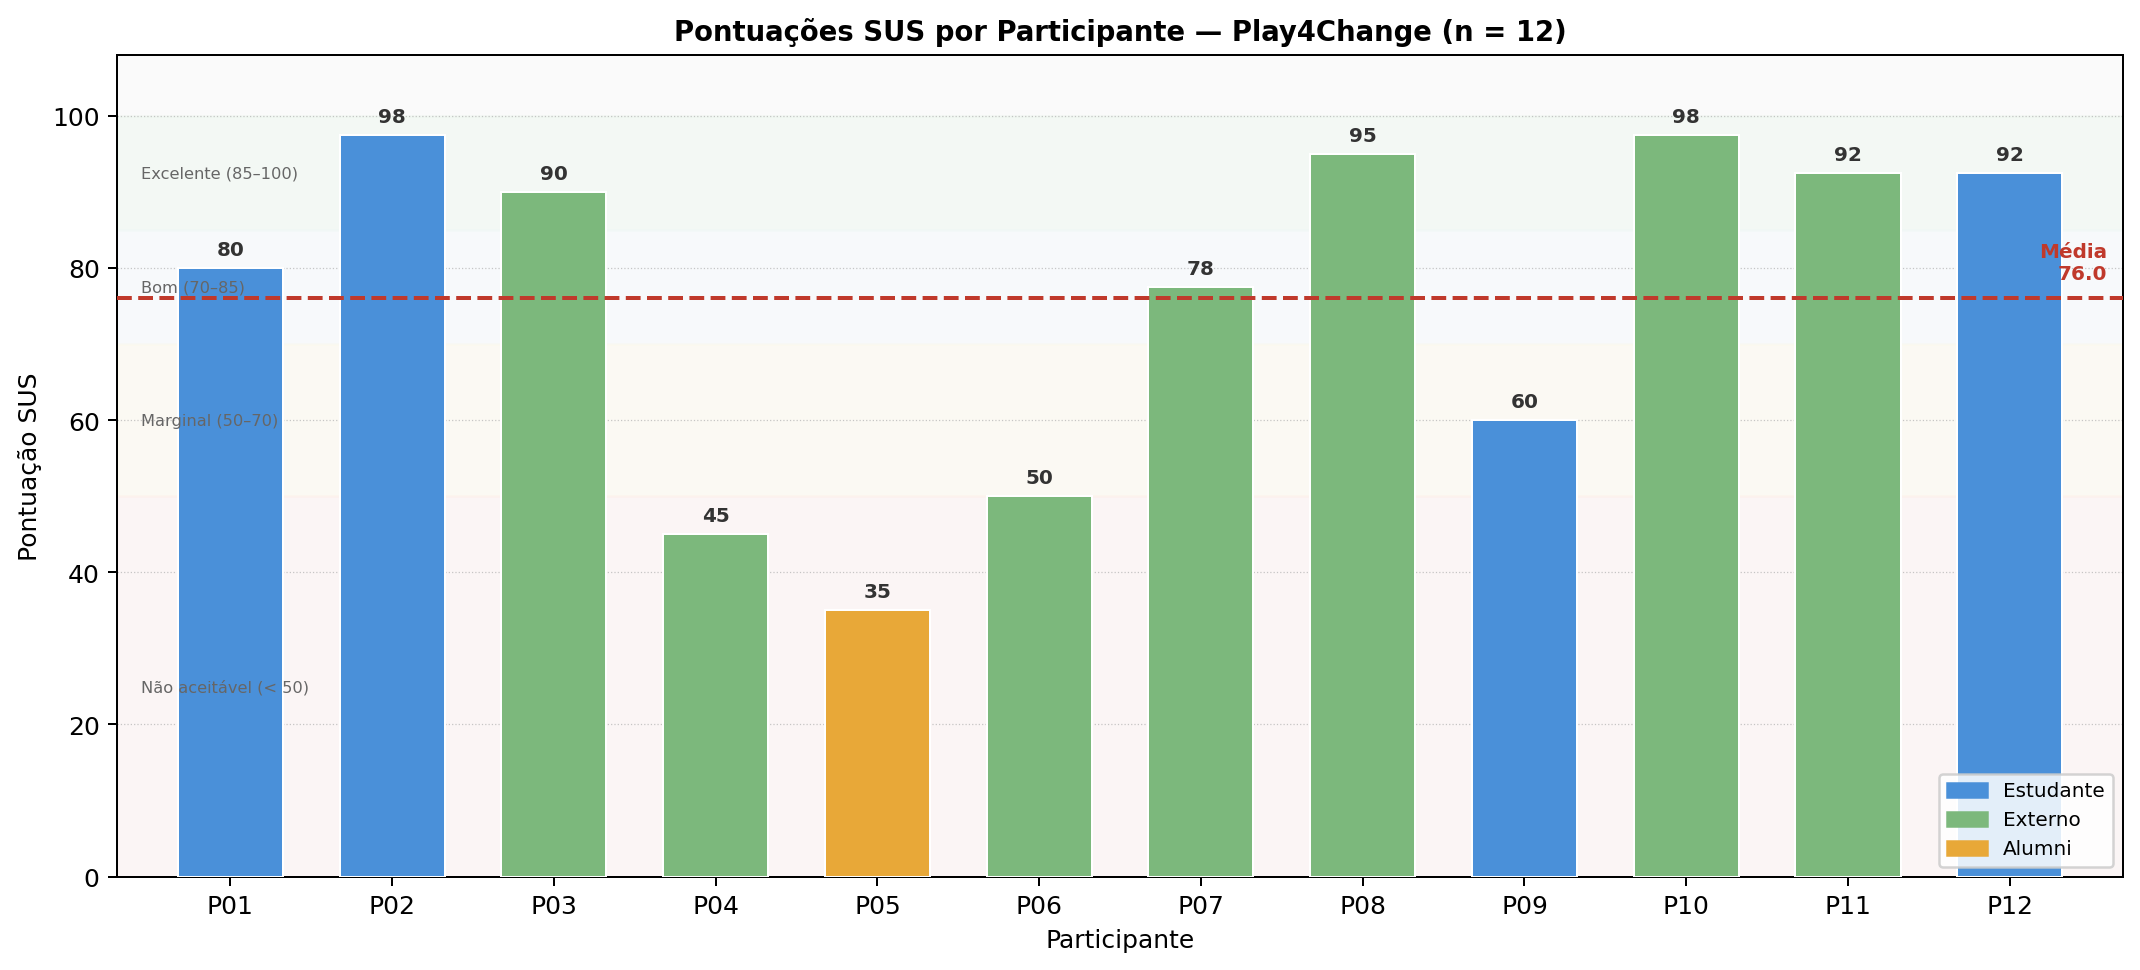
\includegraphics[width=\textwidth]{./figures/chart-sus.png}
\caption{Distribuição das pontuações SUS por participante (\textit{n}~=~12). A linha tracejada indica a média (76,0). As bandas de cor distinguem as quatro categorias: Excelente ($\geq$85), Bom (70–85), Marginal (50–70) e Não aceitável ($<$50).}
\label{fig:chart-sus}
\end{figure}

A média de 76,0 situa-se na categoria \textit{Bom} (70–85); a mediana de 85,0 marca a fronteira com \textit{Excelente}. A discrepância reflecte dois \textit{outliers} (P04~=~45, P05~=~35) que puxam a média para baixo --- sem eles, a média sobe para 83,25. Seis participantes (50\%) obtiveram \textit{Excelente}, dois \textit{Bom}, dois \textit{Marginal} e dois \textit{Não aceitável}. A avaliação global obteve uma média de 4,25 em 5.

As declarações de envolvimento (Tabela~\ref{tab:sus-engagement}) mostram o design visual como a mais bem pontuada (4,33) e o encorajamento a regressar diariamente como a mais baixa (3,92), sugerindo margem de melhoria na retenção.

\begin{table}[htb]
\centering
\caption{Médias das declarações de envolvimento (escala Likert 1–5, \textit{n}~=~12).}
\label{tab:sus-engagement}
\begin{tabular}{@{}lr@{}}
\toprule
\textbf{Declaração} & \textbf{Média} \\
\midrule
A aplicação motivou-me a aprender sobre educação cívica / cidades inteligentes & 3,83 \\
Os desafios pareceram relevantes para problemas do mundo real                  & 4,00 \\
O design visual e a estética do jogo foram apelativos                         & 4,33 \\
Senti-me encorajado/a a regressar e completar desafios diariamente            & 3,92 \\
\midrule
Os caminhos de aprendizagem IA adaptaram-se eficazmente ao meu desempenho     & 4,08 \\
\bottomrule
\end{tabular}
\end{table}

\subsection{Análise Qualitativa} \label{sec:usab-qualitativa}

As respostas abertas revelaram pontos fortes e oportunidades de melhoria consistentes.

\textbf{Pontos fortes.} A explicação adaptativa após resposta errada foi apontada como melhor funcionalidade por quatro participantes; a intuitividade da interface por outros quatro; e a adaptabilidade da IA ao desempenho individual por três. Os desafios diários e a relevância das questões foram igualmente referidos positivamente.

\textbf{Problemas técnicos.} A mais grave foi uma \textit{race condition} visual no caminho de consolidação: a resposta era marcada correta e, meio segundo depois, aparecia como errada. Foram também reportados a barra de pesquisa oculta durante a inserção de e-mail, respostas corretas marcadas intermitentemente como erradas, e questões repetidas em caminhos alternativos. Os dois participantes com pontuações mais baixas (P04, P05) apontaram ainda a confusão causada pela transição abrupta para um novo desafio após resposta errada, sem explicação --- comportamento que ocorre antes de a sessão de \textit{struggle} ser criada.

\textbf{Perfis de afinidade tecnológica.} A observação direta revelou uma segunda linha de segmentação, além do vínculo institucional (Tabela~\ref{tab:sus-scores}): P04 e P05, os dois \textit{outliers} negativos, pertencem a um perfil de utilização tecnológica mínima, sugerindo que a sua pontuação reflecte não só o bug de transição identificado acima, mas também uma dificuldade de base com aprendizagem digital autónoma --- precisamente o perfil que mais beneficiaria do Play4Change (retomada em §\ref{sec:trabalho-futuro}).

\textbf{Sugestões de melhoria.} As mais recorrentes foram funcionalidades sociais (amigos, tabelas de classificação), diversificação de tópicos, maior concisão das explicações IA em mobile, e personalização geográfica das questões por localização.

\textbf{Conclusão da avaliação.} Os resultados SUS indicam usabilidade global \textit{Bom}, com a maioria dos participantes a classificar o sistema como \textit{Excelente}. Os dois \textit{outliers} convergem num problema de comunicação de estado após erro, mitigável com uma transição animada, mas reflectem também uma barreira de entrada mais alta para o perfil de menor afinidade tecnológica.
